%!TEX TS-program = xelatex
%Version 3.1 December 2024
% Springer Nature manuscript prepared for Environmental Science and Pollution Research
% Figures and supporting files are supplied separately at the same folder level.

\documentclass[pdflatex,sn-basic]{sn-jnl}

% Standard packages supplied by the December 2024 Springer Nature template.
\usepackage{graphicx}
\usepackage{multirow}
\usepackage{amsmath,amssymb,amsfonts}
\usepackage{amsthm}
\usepackage[title]{appendix}
\usepackage{xcolor}
\usepackage{textcomp}
\usepackage{manyfoot}
\usepackage{booktabs}
\usepackage{algorithm}
\usepackage{algorithmicx}
\usepackage{algpseudocode}
\usepackage{listings}
\usepackage{longtable}
\usepackage{calc}
\usepackage{array}
\newcounter{none}

\raggedbottom

\begin{document}

\title[Batch level gypsum screening]{A public data decision support tool for batch level triage and pretreatment routing of post consumer gypsum plasterboard}

\author[1,2]{\fnm{Junjie} \sur{Zhang}}\email{junjiezhang2024@shisu.edu.cn}

\author*[3]{\fnm{Yujue} \sur{Cao}}\email{yujuecao\_real@126.com; caoyujue@cuhk.edu.cn}

\affil[1]{\orgdiv{Shanghai Academy of Global Governance \& Area Studies}, \orgname{Shanghai International Studies University}, \orgaddress{\city{Shanghai}, \postcode{201620}, \country{China}}}

\affil[2]{\orgdiv{School of Economics and Finance}, \orgname{Shanghai International Studies University}, \orgaddress{\city{Shanghai}, \postcode{201620}, \country{China}}}

\affil[3]{\orgdiv{School of Public Policy}, \orgname{The Chinese University of Hong Kong}, \orgaddress{\city{Shenzhen}, \postcode{518172}, \country{China}}}

\abstract{Post consumer gypsum plasterboard recycling requires consistent routing when feed records are incomplete. This public data study develops a decision support tool that converts traceable sources and registered parameter intervals into a dry mass balance, mass triage screen and sequential measurement checklist. For a normalized 1,000 kg dry equivalent input, four scenarios are evaluated over 32 parameter corners. C0 yields 734.026 kg at the base point and 662.592--739.200 kg across corners; all corners pass the primary mass screen. C1 is a boundary case, C2 is routed to pretreatment and recheck because of a visible nonhazardous contamination flag, and C3 exits at the safety gate. C0--C2 require confirmation of calcium sulfate or chemical purity, total organic carbon, moisture, salts and pH. The 0.84 composition share and the 0.80--0.88 German process range are retained as non equivalent denominator variants. The tool delivers a reproducible routing record, not product certification, empirical prevalence or a life cycle assessment.}

\keywords{gypsum plasterboard, construction and demolition waste, recycled gypsum, batch screening, pretreatment, mass balance, public data}

\maketitle

\section*{Author identifiers}
Junjie Zhang: \url{https://orcid.org/0009-0004-8821-4018}; Yujue Cao: \url{https://orcid.org/0000-0001-9911-9746}.

\section{Introduction}\label{introduction}

Gypsum plasterboard is a technically attractive construction and demolition waste stream because the calcium sulfate phase can be processed into secondary gypsum \citep{jimenezRivero2016,jimenezRivero2017Factors,pantini2019,morsali2024,cristobal2024,iso14040,iso14044}. At a recovery facility, operators must decide whether a recorded batch should be routed to safety exclusion, pretreatment, mass triage or product chemistry acceptance when the input basis, contamination composition and moisture are incomplete. Paper fibres, wood, coatings, mineral fragments, metals, soluble salts, moisture and hazardous materials have different routing consequences. A single residual mass fraction therefore cannot represent the complete acceptance decision. The present study treats composition, moisture, visible contamination and safety information as separate routing fields.

Previous studies on gypsum recycling can be grouped into three connected evidence layers. Process specific studies report separation, purification and product responses across industrial, laboratory and material development settings \citep{jimenezRivero2017Best,pedrenoRojas2020,weimann2021,castroDiaz2024Acid,castroDiaz2024Wastewater,castroDiaz2023Dataset,perezGalvez2025,pedrenoRojas2025Wood,capasso2025,castroDiaz2023Preprint,atienza2025,jimenezRivero2017Characterization,rodrigoBravo2025,nowak2024,mizuishi2026}. Quality criteria, waste legislation and technical guidance define the analytical fields and route conditions used to interpret those results \citep{eurogypsum2024,bundesverband2013,en15936_2022,eu2008WasteDirective,eu2024WasteShipments,reetsch2024,jrcEndOfWaste,tris2025,ec2024EndWasteMetadata,ec2020Bemp,jrcCdw,ecWasteFramework,deloitte2017}. Circular economy studies and project or dataset records add supply chain, programme and macro data context \citep{mhlanga2025Business,mhlanga2025Implementation,lifeGypsumProject,eurostatW121,eurostatEnergyPrices,jrcElectricityFactors,cineA_GtoG}. Together, these sources establish the value of recycling and the heterogeneity of feed and process conditions, but they do not provide a single harmonized batch record linking input composition, dry mass yield, product chemistry, safety flags, energy, rejects and acceptance outcome. The practical gap is therefore an operational one: facilities need a traceable protocol that identifies the next defensible action and the measurements required for a qualified product decision.

The distinction between an engineering screen and a product acceptance test is central. Eurogypsum's quality document specifies total organic carbon, calcium sulfate composition and other product criteria \citep{eurogypsum2024}, while EN 15936:2022 defines TOC determination as a dry combustion measurement \citep{en15936_2022}. The model therefore treats total organic carbon and calcium sulfate purity as product basis measurements, while mass fractions provide a transparent triage layer that prioritizes inspection or pretreatment.

Environmental interpretation follows the same boundary discipline. Published route level climate results are retained as external context, while the present analysis reports direct process inventory components using an explicit functional unit and foreground boundary \citep{cristobal2024,iso14040,iso14044}.

The research question is:

\begin{quote}
Under fixed safety and product quality requirements, what can an interval based public data screen identify about batch routing, required confirmatory measurements and process mass output?
\end{quote}

Three subsidiary questions follow:

\begin{enumerate}


\item
  Do the registered parameter ranges, equations and derived outputs form one internally consistent mass balance?
\item
  How does a sequential safety first policy differ from a mass proxy only policy when chemical acceptance variables are unavailable?
\item
  How do denominator choice, registered parameter bounds and direct process energy components constrain interpretation of a possible closed loop route?
\end{enumerate}

The contribution is a measurement aligned decision support tool. It is designed for facility records and public data screening. It (i) makes dry and wet denominators explicit, (ii) keeps mass triage variables separate from TOC and calcium sulfate acceptance, (iii) routes nonhazardous visible contamination to pretreatment and recheck, (iv) identifies the five confirmatory fields required before a qualified product claim can be made and (v) provides a reproducible decision log for checking the screen against external public records. Its operational output is a prioritized next action and a record of the fields required for product acceptance. Scope Box 1 defines the primary output and evidence basis.

\begin{quote}
\textbf{Box 1 \textbar{} Scope and primary output}

This study uses publicly available data and computational screening for batch routing and measurement prioritization. It delivers four operational outputs: a dry mass balance, a mass triage stability assessment, a pretreatment versus safety exclusion rule, and a five field chemistry panel required for a qualified product claim. The primary output is dry gypsum equivalent and routing status. Product acceptance is represented by the product basis chemistry fields required by the selected receiving route, while \(P_{mass}\) and \(O_{mass}\) serve as triage indicators. The resulting decision log identifies the next measurement or route for each registered scenario and supports subsequent physical verification and facility records.
\end{quote}

\section{Materials and methods}\label{materials-and-methods}

\subsection{Study design and evidence classes}\label{study-design-and-evidence-classes}

This is a public data computational study within the boundary stated in Scope Box 1. The primary inputs are public official data, public research data deposits, open papers and public technical documents. Official Eurostat waste and energy datasets provide macro context and price metadata, while batch quality observations remain source specific \citep{eurostatW121,eurostatEnergyPrices}. The source manifest records the source location, retrieval date, extraction note, parameter role and limitation. A public data availability audit distinguishes four core variable groups found in public form, four partial groups and four missing batch level groups. These missing groups define the public evidence gap: harmonized batch composition, moisture and storage condition, contamination stratified yield, and acceptance linked product chemistry. They also identify the fields needed when a facility extends the public screening record. No additional sampling, laboratory campaign or participant data collection is part of this study.

The analysis distinguishes four evidence types:

\begin{itemize}

\item
  a researcher defined scenario is a transparent model input;
\item
  a published process range is an external process anchor with its original denominator;
\item
  a batch observation is a selected observation from its source study and is not an EU population estimate;
\item
  a technical criterion is a measurement requirement or screening reference, not necessarily a legal or contractual rule.
\end{itemize}

This classification prevents a scenario corner, a country electricity factor and a repeated observation from being counted as independent public records.

\subsection{Registered parameter set}\label{registered-parameter-set}

The analysis uses a single parameter registry. The normalized reference flow is 1,000 kg dry equivalent candidate input. The board bearing share (b=0.84) is a JRC modeled composition scenario \citep{cristobal2024}, not an observed EU batch prevalence. The registered base values and bounds are:

\small
\begin{longtable}[]{@{}
  >{\raggedright\arraybackslash}p{(\linewidth - 12\tabcolsep) * \real{0.1154}}
  >{\raggedleft\arraybackslash}p{(\linewidth - 12\tabcolsep) * \real{0.1538}}
  >{\raggedleft\arraybackslash}p{(\linewidth - 12\tabcolsep) * \real{0.1538}}
  >{\raggedleft\arraybackslash}p{(\linewidth - 12\tabcolsep) * \real{0.1538}}
  >{\raggedleft\arraybackslash}p{(\linewidth - 12\tabcolsep) * \real{0.1538}}
  >{\raggedleft\arraybackslash}p{(\linewidth - 12\tabcolsep) * \real{0.1538}}
  >{\raggedright\arraybackslash}p{(\linewidth - 12\tabcolsep) * \real{0.1154}}@{}}
\caption{Registered parameter intervals and routing flags}\\
\toprule\noalign{}
\begin{minipage}[b]{\linewidth}\raggedright
Scenario
\end{minipage} & \begin{minipage}[b]{\linewidth}\raggedleft
\(y\) (conditional dry yield)
\end{minipage} & \begin{minipage}[b]{\linewidth}\raggedleft
\(p\) (paper fraction)
\end{minipage} & \begin{minipage}[b]{\linewidth}\raggedleft
\(c\) (coating or wood fraction)
\end{minipage} & \begin{minipage}[b]{\linewidth}\raggedleft
\(r\) (mineral residue fraction)
\end{minipage} & \begin{minipage}[b]{\linewidth}\raggedleft
\(w_{out}\) (free product moisture)
\end{minipage} & \begin{minipage}[b]{\linewidth}\raggedright
Routing flag
\end{minipage} \\
\midrule\noalign{}
\endhead
\bottomrule\noalign{}
\endlastfoot
C0 clean selective & 0.88 {[}0.80, 0.88{]} & 0.005 {[}0, 0.01{]} & 0.001 {[}0, 0.002{]} & 0.001 {[}0, 0.002{]} & 0.02 {[}0, 0.04{]} & no hazard; no visible flag \\
C1 moderate selective & 0.85 {[}0.80, 0.88{]} & 0.02 {[}0, 0.04{]} & 0.01 {[}0, 0.02{]} & 0.01 {[}0, 0.02{]} & 0.10 {[}0, 0.20{]} & no hazard; no visible flag \\
C2 high contamination & 0.65 {[}0.55, 0.75{]} & 0.05 {[}0, 0.10{]} & 0.05 {[}0, 0.10{]} & 0.05 {[}0, 0.10{]} & 0.20 {[}0, 0.40{]} & visible flag \\
C3 hazardous exclusion & 0 {[}0, 0{]} & 0 {[}0, 0{]} & 0 {[}0, 0{]} & 0 {[}0, 0{]} & 0 {[}0, 0{]} & hazard flag \\
\end{longtable}
\normalsize

Here \(y\) is a conditional dry process output yield on the registered board reference flow; \(p\), \(c\) and \(r\) are retained dry mass fractions of paper, coating or wood and mineral residue in the process output; and \(w_{out}\) is free moisture in the product output. It is not incoming moisture. The three C0 non yield upper bounds are heterogeneous.

\textbf{Denominator declaration.} The primary model uses the JRC modeled board bearing share \(b=0.84\) for all scenario outputs. The Weimann range of 0.80 to 0.88 (Weimann et al., 2021) is retained as an external process anchor for denominator illustration only. It is not multiplied by 0.84 in the interval enumeration because the two sources define different input bases. Figure 1 makes this distinction visible: the left panel is the primary model balance and the right panel is an external range, not a second observed process stage.

\subsection{Process stages and mass denominators}\label{process-stages-and-mass-denominators}

The mass balance uses a normalized dry equivalent reference to avoid silently treating water as a conservative mass component. For an as received batch, the correct conversion is:

\[
M_{in,dry}=M_{in,wet}(1-w_{in}),qquad
y_{dry}=\frac{M_{product,dry}}{M_{in,dry}}.
\]

Because no harmonized \(w_{in}\) field is available in the public data, the primary model does not infer an as received wet input. It sets \(M_{in,dry}=1{,}000\) kg as a normalized reference. Product moisture is reported separately:

\[
M_{product,wet}=\frac{M_{product,dry}}{1-w_{out}}.
\]

This conversion is an ancillary wet product calculation, not a statement that free water is recovered or conserved.

The model stages are:

\[
\begin{aligned}
M_{board,dry} &= bM_{in,dry},\\
M_{process,dry} &= M_{board,dry}y,\\
M_{paper} &= M_{process,dry}p,\\
M_{coating/wood} &= M_{process,dry}c,\\
M_{mineral} &= M_{process,dry}r,\\
G_{dry} &= M_{process,dry}(1-p-c-r),\\
M_{board,loss} &= M_{board,dry}(1-y).
\end{aligned}
\]

The 0.84 composition share and the 0.80 to 0.88 Weimann process range (Weimann et al., 2021) are therefore reported in two denominator variants. In the first, the 0.84 share is a modeled composition fraction and the yield is applied conditionally to the board bearing reference stream. In the second, the Weimann range is retained as a study specific output per post consumer input, without multiplication by 0.84. The two numbers are not treated as two stages of one empirically observed process unless a matched process study establishes that interpretation.

\subsection{Quality measurement hierarchy}\label{quality-measurement-hierarchy}

The model has two distinct quality layers. The first is a mass triage screen. It calculates:

\[
P_{mass}=\frac{G_{dry}}{M_{process,dry}}=1-p-c-r,qquad
O_{mass}=p+c.
\]

\(P_{mass}\) is a residual mass purity proxy and \(O_{mass}\) is a retained organic mass proxy. The diagnostic limits are used as triage limits: \(O_{mass}\leq0.02\), \(p+c+r\leq0.20\) and \(w_{out}\leq0.10\). Chemical acceptance remains a separate product basis decision.

The second layer is chemical and product acceptance. It requires measurements on the product basis specified by the selected receiving route: calcium sulfate composition or chemical purity, total organic carbon, free moisture, soluble chloride or other salts where relevant, pH and any hazard specific test \citep{eurogypsum2024,bundesverband2013}. Eurogypsum's 2\% criterion is a TOC criterion example; the mass proxy \(O_{mass}\) is not a substitute for the measured TOC value required by the receiving route. The same logic applies to calcium sulfate purity: a residual fraction after subtracting estimated contaminants cannot be called a CaSO4 assay.

\subsection{Screening policies and outputs}\label{screening-policies-and-outputs}

Three policies are compared at the scenario level:

\begin{itemize}

\item
  \texttt{mass\ proxy\ only} uses hazard, visibility, component fractions and moisture but has no chemical acceptance fields. Its product acceptance status is therefore unsupported.
\item
  \texttt{sequential\ safety\ first} checks hazard, then visible nonhazardous contamination, then the mass triage screen, then targeted processing or recheck where needed, followed by a five field chemical panel: CaSO4 or chemical purity, TOC, product moisture, chloride and pH.
\item
  \texttt{all\ confirmatory\ panel\ after\ safety\ gate} applies the same chemical panel to every nonhazardous branch after the safety checks.
\end{itemize}

The primary outputs are the required confirmatory field count per registered scenario, the product routing state and the dry mass output interval. When a public record reports matched input and product quantities, qualified recovery is calculated as:

\[
Y_{qualified,b,r}=\frac{\sum_k M^{dry}_{out,b,r,k}\,\mathbf{1}\{\text{product }k\text{ meets the receiving specification}\}}{M^{dry}_{in,b}}.
\]

The matched product fields needed to estimate \(Y_{qualified,b,r}\) are listed in the public batch observation schema; they are not inferred from the public scenario registry and are not available as a harmonized panel in this study.

\subsection{Interval enumeration and model structure audit}\label{interval-enumeration-and-model-structure-audit}

For each scenario, all \(2^5=32\) combinations of the lower and upper registered values of \((y,p,c,r,w_{out})\) are enumerated. The rectangle is a feasibility envelope, not a joint probability distribution. In particular, a high contamination scenario with several zero lower bounds is a stress test envelope and not a claim that clean corners occur frequently in high contamination feed.

The audit records the minimum and maximum mass output, mass proxy margins and triage status. It does not interpret corner fractions as empirical probabilities. It also records algebraic effects. Yield changes output mass but cancels from the dry composition proxies. The mass purity relation is mechanically linked to total non gypsum mass. These are properties of the equations, not empirical claims about the value of a measurement.

\subsection{Direct energy boundary}\label{direct-energy-boundary}

The direct process inventory is retained because it is technically relevant and available in an open Spanish study \citep{pedrenoRojas2020}: 60.35 kWh electricity, 13.59 m3 natural gas and 0.90 L diesel per tonne of process product. The present paper reports the inventory components and, for electricity, the dated 2021 JRC country factor sensitivity \citep{jrcElectricityFactors}:

\[
I_{el,c}=60.35\,F_{el,c},
\]

where \(F_{el,c}\) is the selected country life cycle electricity factor in kg CO2 equivalent per kWh. The JRC 66 to 104 kg CO2 equivalent per tonne gypsum benchmark \citep{cristobal2024} is retained only as an external published result. It is not subtracted from \(I_{el,c}\), because the benchmark already represents a route level net saving with a different functional unit and substitution boundary. No net climate headroom or country level avoided emission claim is made.

\section{Results}\label{results}

\subsection{Mass-screen stability and parameter consistency}\label{mass-screen-stability-and-parameter-consistency}

The primary engineering output is a stable C0 mass-screen envelope. Across all 32 registered C0 corners, the dry gypsum equivalent remains between 662.592 and 739.200 kg, the mass purity proxy remains at or above 0.986 and the retained organic mass proxy remains at or below 0.012. All 32 corners pass the primary mass triage screen. These results are generated from the heterogeneous bounds \(p\leq0.01\), \(c\leq0.002\), \(r\leq0.002\) and \(w_{out}\leq0.04\) in the registered parameter set.

At the base point, the model outputs are 734.026 kg dry gypsum equivalent for C0, 685.440 kg for C1 and 464.100 kg for C2. The corresponding gross dry process outputs are 739.200, 714.000 and 546.000 kg. The ancillary wet product conversions are 754.286, 793.333 and 682.500 kg. C3 terminates at the hazard gate. The C0 envelope is therefore a reproducible mass-screen candidate for an orderly confirmatory chemistry workflow. Operationally, every registered C0 corner reaches the same next step: chemistry confirmation. The model assigns this common measurement priority; test time and cost require separate facility records.

\subsection{Decision rules: pretreatment versus safety exclusion}\label{decision-rules-pretreatment-versus-safety-exclusion}

The routing hierarchy produces a clear operational distinction. Confirmed hazard sends a batch to a safety exclusion or other authorized route before product interpretation. A visible nonhazardous contaminant sends the batch to a pretreatment and recheck branch. A batch without either flag proceeds through mass triage and then the five field chemical panel. This rule gives C2 a recoverable process branch while preserving a hard safety gate for C3.

For a facility quality control workflow, the protocol records the C2 branch as pretreat and recheck rather than converting a visible contamination flag into final rejection. The C3 branch terminates at the hazard gate. Figure 3 displays the hierarchy from safety screening to product acceptance.

\subsection{Scenario outputs and confirmatory chemistry requirements}\label{scenario-outputs-and-confirmatory-chemistry-requirements}

The base scenario results are summarized below. The mass screen is an operational triage layer, while product acceptance uses the receiving route's chemistry panel.

\scriptsize
\begin{longtable}[]{@{}
  >{\raggedright\arraybackslash}p{(\linewidth - 10\tabcolsep) * \real{0.1429}}
  >{\raggedleft\arraybackslash}p{(\linewidth - 10\tabcolsep) * \real{0.1905}}
  >{\raggedleft\arraybackslash}p{(\linewidth - 10\tabcolsep) * \real{0.1905}}
  >{\raggedleft\arraybackslash}p{(\linewidth - 10\tabcolsep) * \real{0.1905}}
  >{\raggedright\arraybackslash}p{(\linewidth - 10\tabcolsep) * \real{0.1429}}
  >{\raggedright\arraybackslash}p{(\linewidth - 10\tabcolsep) * \real{0.1429}}@{}}
\caption{Scenario level mass triage and routing outputs}\\
\toprule\noalign{}
\begin{minipage}[b]{\linewidth}\raggedright
Scenario
\end{minipage} & \begin{minipage}[b]{\linewidth}\raggedleft
Dry gypsum equivalent (kg)
\end{minipage} & \begin{minipage}[b]{\linewidth}\raggedleft
Mass purity proxy
\end{minipage} & \begin{minipage}[b]{\linewidth}\raggedleft
Organic mass proxy
\end{minipage} & \begin{minipage}[b]{\linewidth}\raggedright
Mass triage
\end{minipage} & \begin{minipage}[b]{\linewidth}\raggedright
Final route status
\end{minipage} \\
\midrule\noalign{}
\endhead
\bottomrule\noalign{}
\endlastfoot
C0 & 734.026 & 0.993 & 0.006 & pass & chemistry confirmation \\
C1 & 685.440 & 0.960 & 0.030 & flag & chemistry confirmation \\
C2 & 464.100 & 0.850 & 0.100 & flag / boundary & pretreat; recheck \\
C3 & 0 & n/a & n/a & n/a & safety / other \\
\end{longtable}
\normalsize

C0 passes the primary mass triage in 32 of 32 corners and the stricter diagnostic limits in 24 of 32 corners. C1 passes 8 of 32 corners under the primary limits and 4 of 32 under the strict limits. C2 passes 4 of 32 corners under each mass triage limit, but its visible nonhazardous flag sends it to pretreatment rather than directly rejecting the final product. C3 terminates at the hazard gate; no product panel is assigned to that branch.

These counts identify the information and routing state created by the registered mass envelope. The mass layer prioritizes the next action, while product acceptance uses measurements on the receiving route's product basis. Thus, \(O_{mass}=p+c\) is used as a mass triage proxy and \(P_{mass}=1-p-c-r\) as a residual mass proxy; TOC and chemical calcium sulfate purity remain separate measurements. In operational terms, C0 can enter the chemistry queue, C1 remains conditional, C2 requires documented pretreatment and recheck, and C3 is assigned to the safety route. The protocol preserves the receiving specification while making the next measurement explicit.

\subsection{Denominator audit and process mass balance}\label{denominator-audit-and-process-mass-balance}

The primary model uses the JRC modeled 0.84 board share \citep{cristobal2024}. Applying that share to the Weimann conditional process range \citep{weimann2021} gives an illustrative 672 to 739.2 kg dry process output per 1,000 kg normalized reference. The Weimann study's own output range is 800 to 880 kg per tonne of its post consumer input definition. These ranges answer different questions and are retained as denominator variants rather than combined process stages. The registered C0 gypsum equivalent, after its retained fractions, is 662.592 to 739.200 kg across the parameter corners. Figure 1 shows the primary model balance alongside the external range.

The denominator declaration is part of the result: the model reports how much dry mass follows from \(b=0.84\) and its registered yields, while the Weimann range remains an external process anchor. Comparison with this screen requires records that report the as received feed, dry input, board bearing fraction, every process output and every reject at each stage.

\begin{figure}[htbp]
\centering
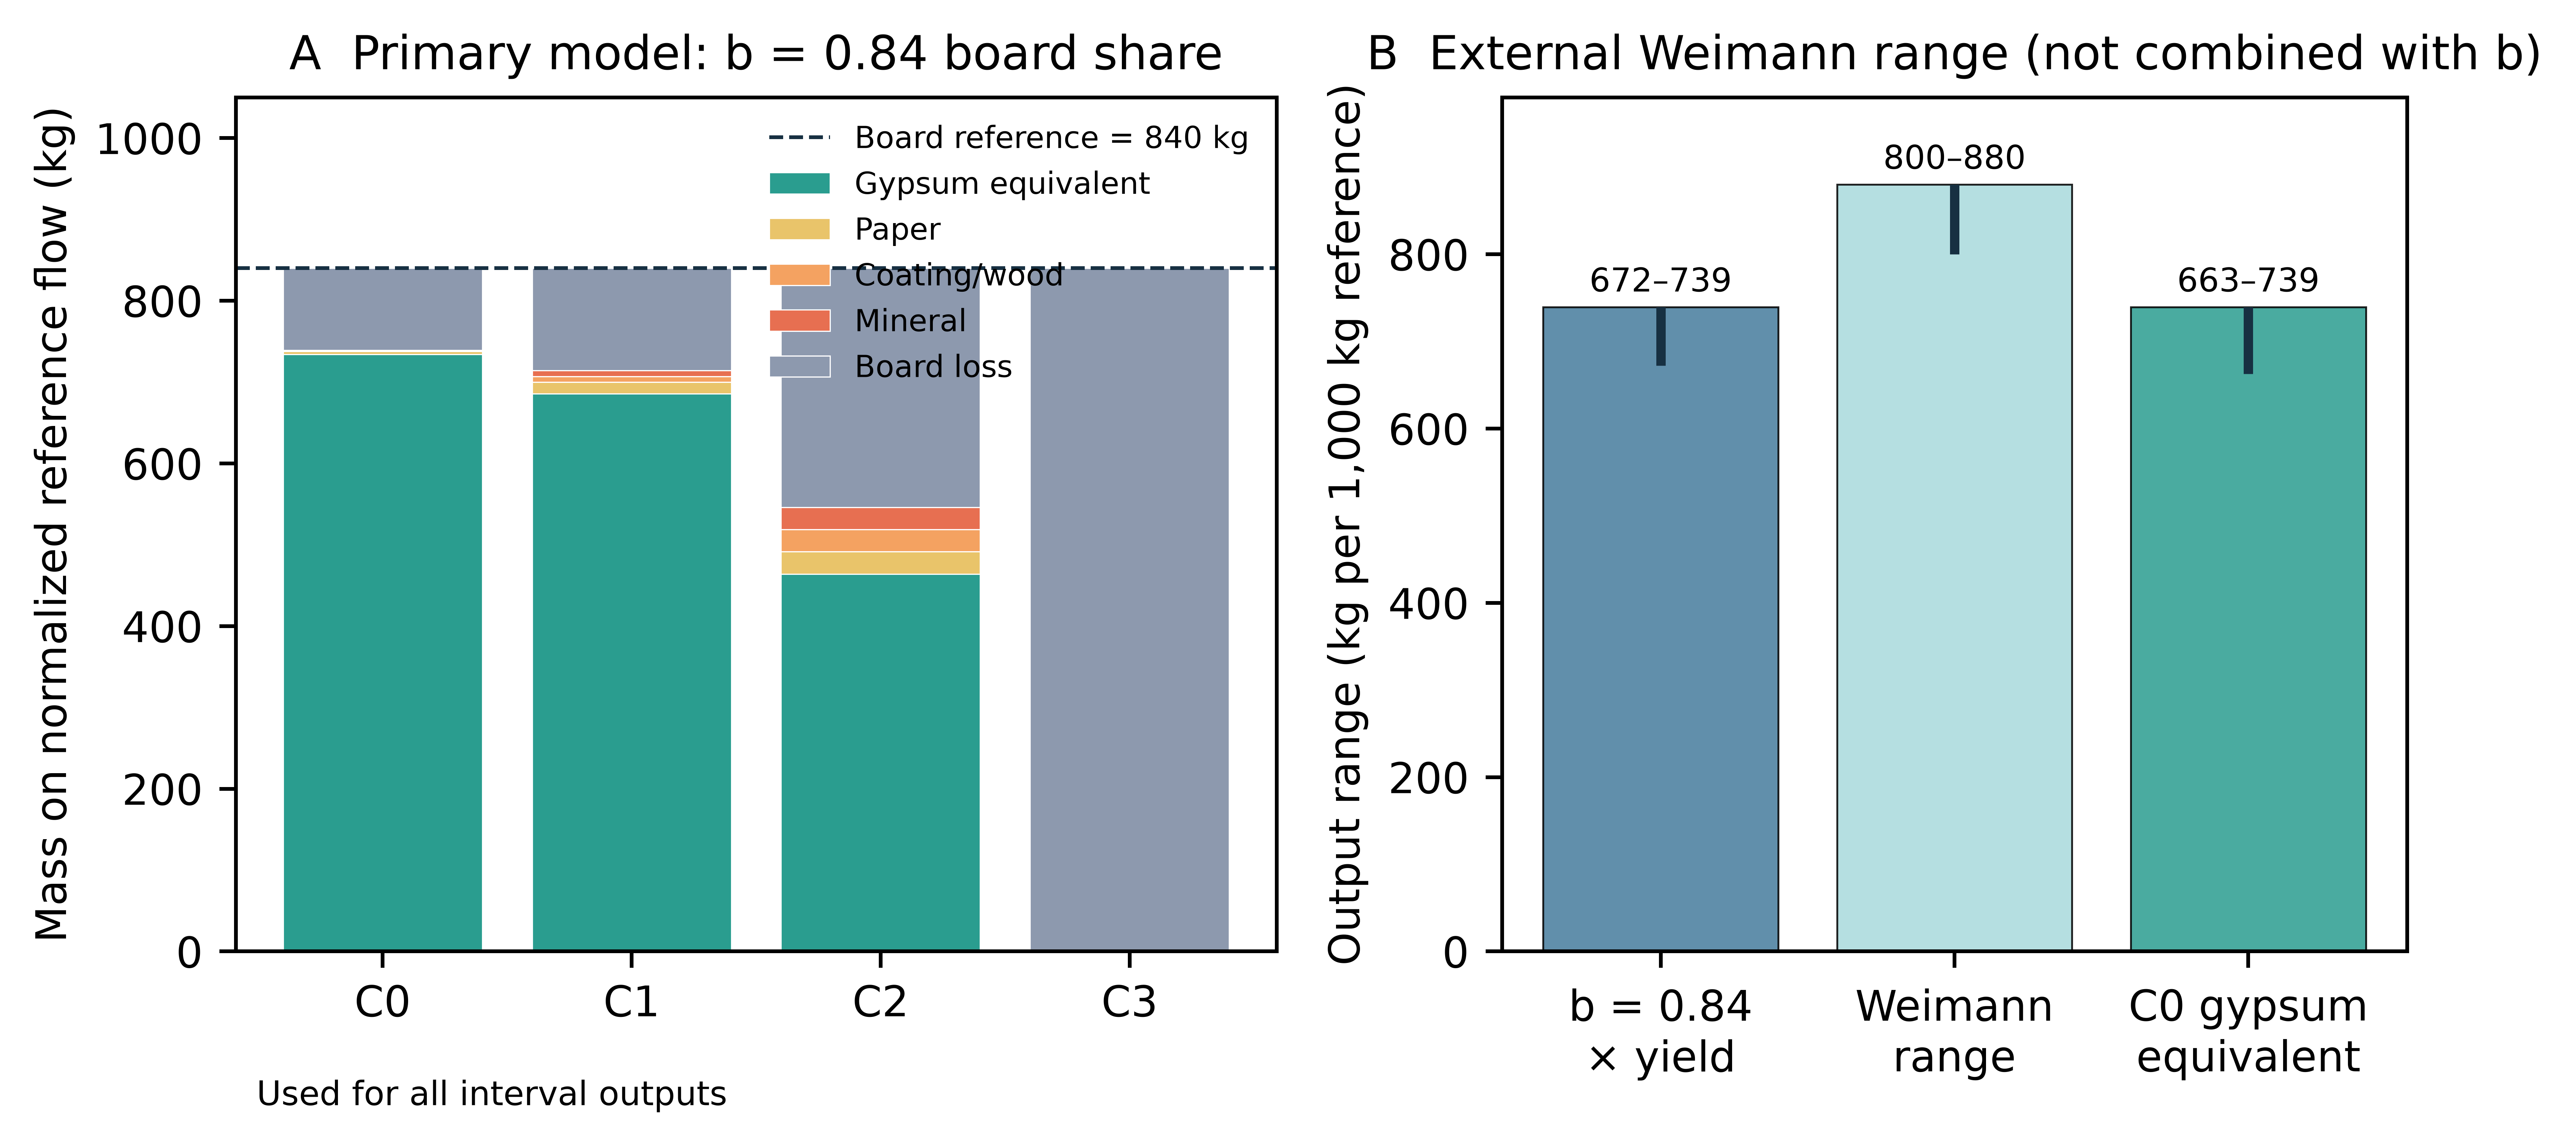
\includegraphics[width=0.96\textwidth]{Fig1_process_mass_balance.png}
\caption{Primary model balance with b = 0.84 and external Weimann range shown as a denominator variant}\label{fig:mass-balance}
\end{figure}



\subsection{Sequential measurement workflow}\label{sequential-measurement-workflow}

The sequential policy assigns five confirmatory fields to C0, C1 and C2, while C3 stops at the hazard branch. The all confirmatory policy also assigns five fields to each nonhazardous branch. The practical output is a safety first ordering rule and a fixed chemistry panel for facility records and public batch reporting; population testing time, cost and error rates require comparable observed records. Figure 2 reports the field counts, and Figure 3 separates safety, pretreatment, mass triage and chemical acceptance.

The mass proxy only policy returns \texttt{UNSUPPORTED\_FOR\_PRODUCT\_ACCEPTANCE} for all scenarios. The sequential policy converts that unsupported state into a specified next action: confirmatory chemistry for C0 and C1, pretreatment and recheck for C2, and safety exclusion for C3.

\begin{figure}[htbp]
\centering
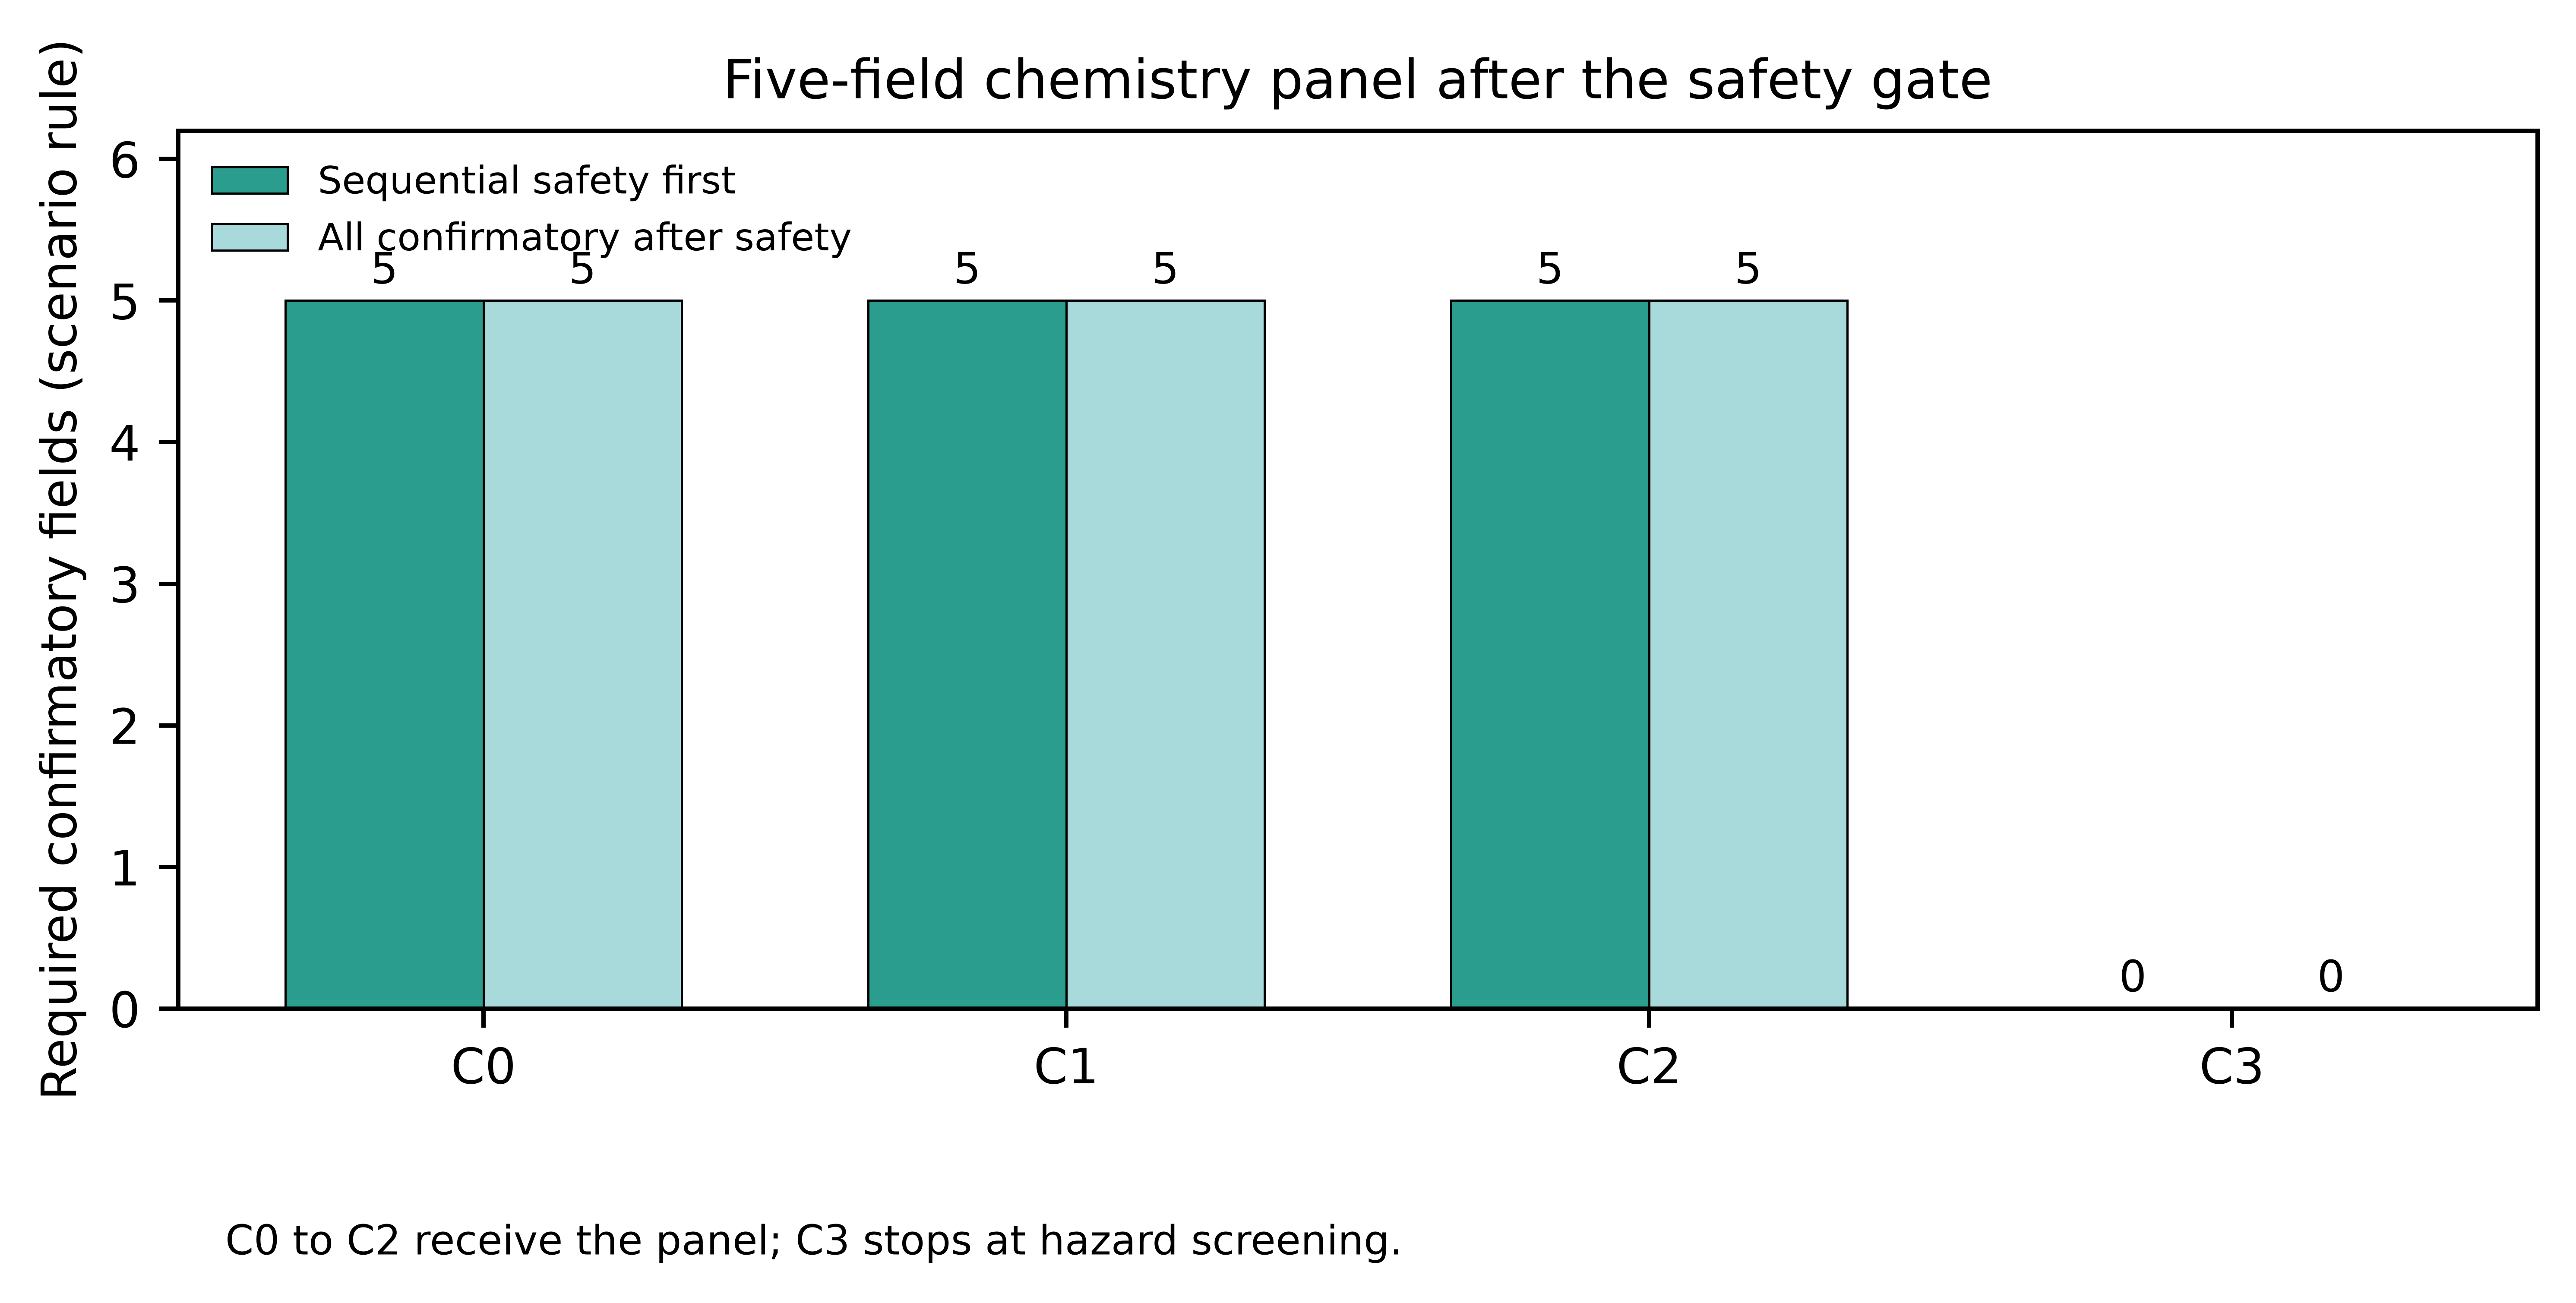
\includegraphics[width=0.96\textwidth]{Fig2_screening_policy_burden.png}
\caption{Five field chemistry panel assigned after the safety gate for C0 to C2}\label{fig:policy-burden}
\end{figure}



\begin{figure}[htbp]
\centering
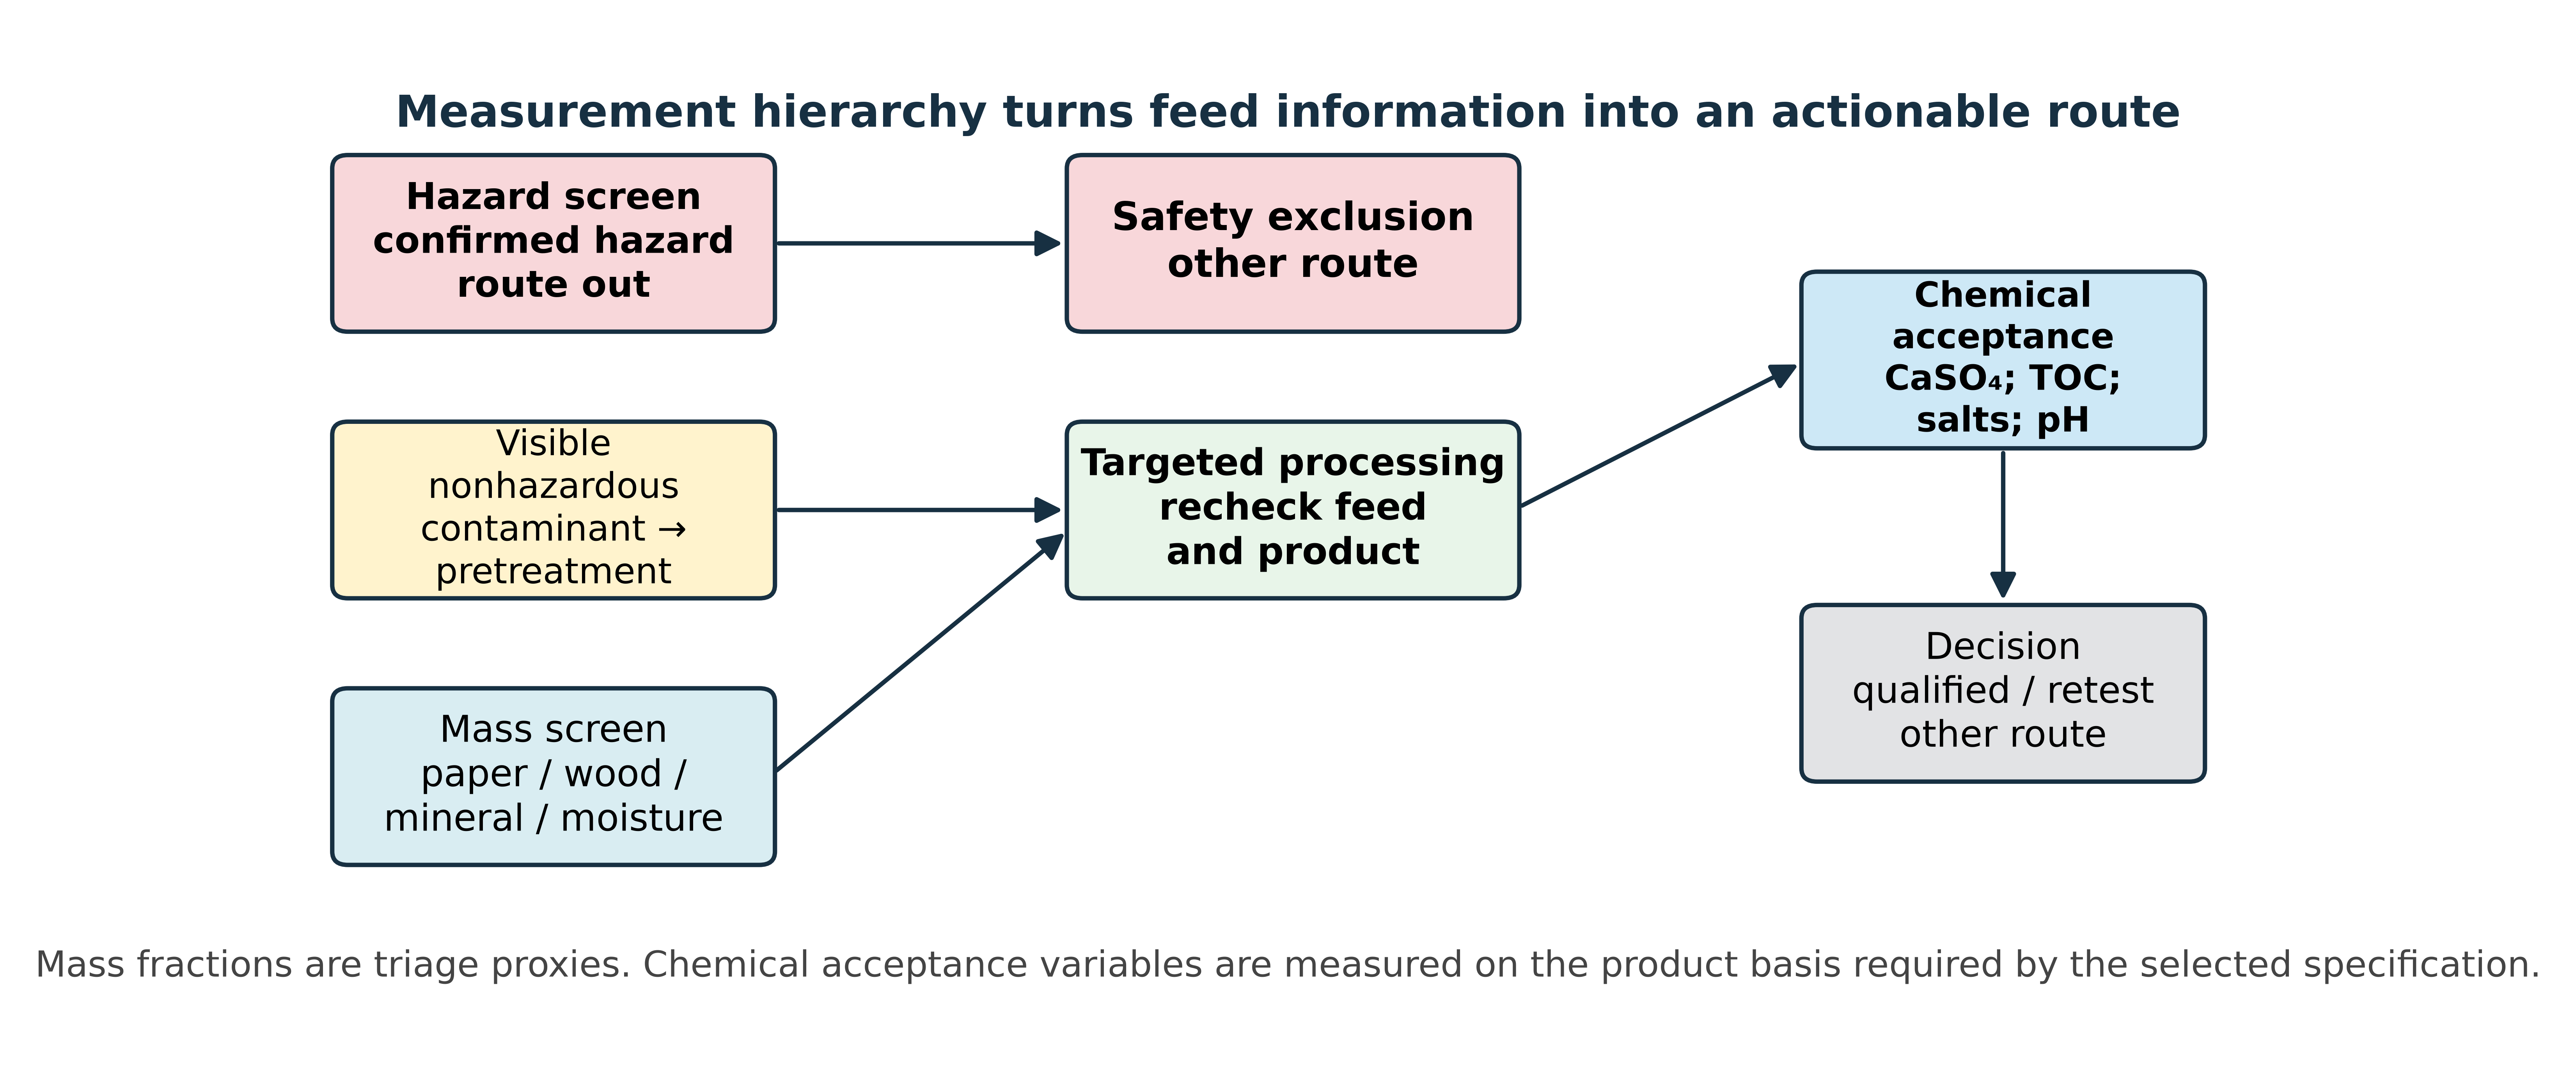
\includegraphics[width=0.96\textwidth]{Fig3_quality_measurement_hierarchy.png}
\caption{Measurement hierarchy from hazard screening to pretreatment, mass triage and chemical acceptance}\label{fig:measurement-hierarchy}
\end{figure}



\subsection{Public observations as module specific anchors}\label{public-observations-as-module-specific-anchors}

The selected UK public data contain chemical purity measurements in the mid 90 wt\% range and an extracted post sieving inorganic impurity scale around 4 to 6 wt\% for selected feed trajectories \citep{castroDiaz2024Acid,castroDiaz2023Dataset}. Figure 4 places these quantities side by side as a module specific external anchor. The records motivate matched measurement of the mass proxy and product chemistry, while their source specific denominators and trajectories are retained. They therefore inform measurement planning rather than a European distribution.

The GtoG and UPM aggregate \citep{lifeGypsumProject,cineA_GtoG} provides a second context with mean moisture 6.91\%, mean reported purity 87.41\% and mean TOC 0.85\% across selected feedstock samples. These aggregate values support planning for matched measurement of moisture, purity and TOC; the source records retain their own measurement definitions rather than supplying a mass component to TOC conversion.

\begin{figure}[htbp]
\centering
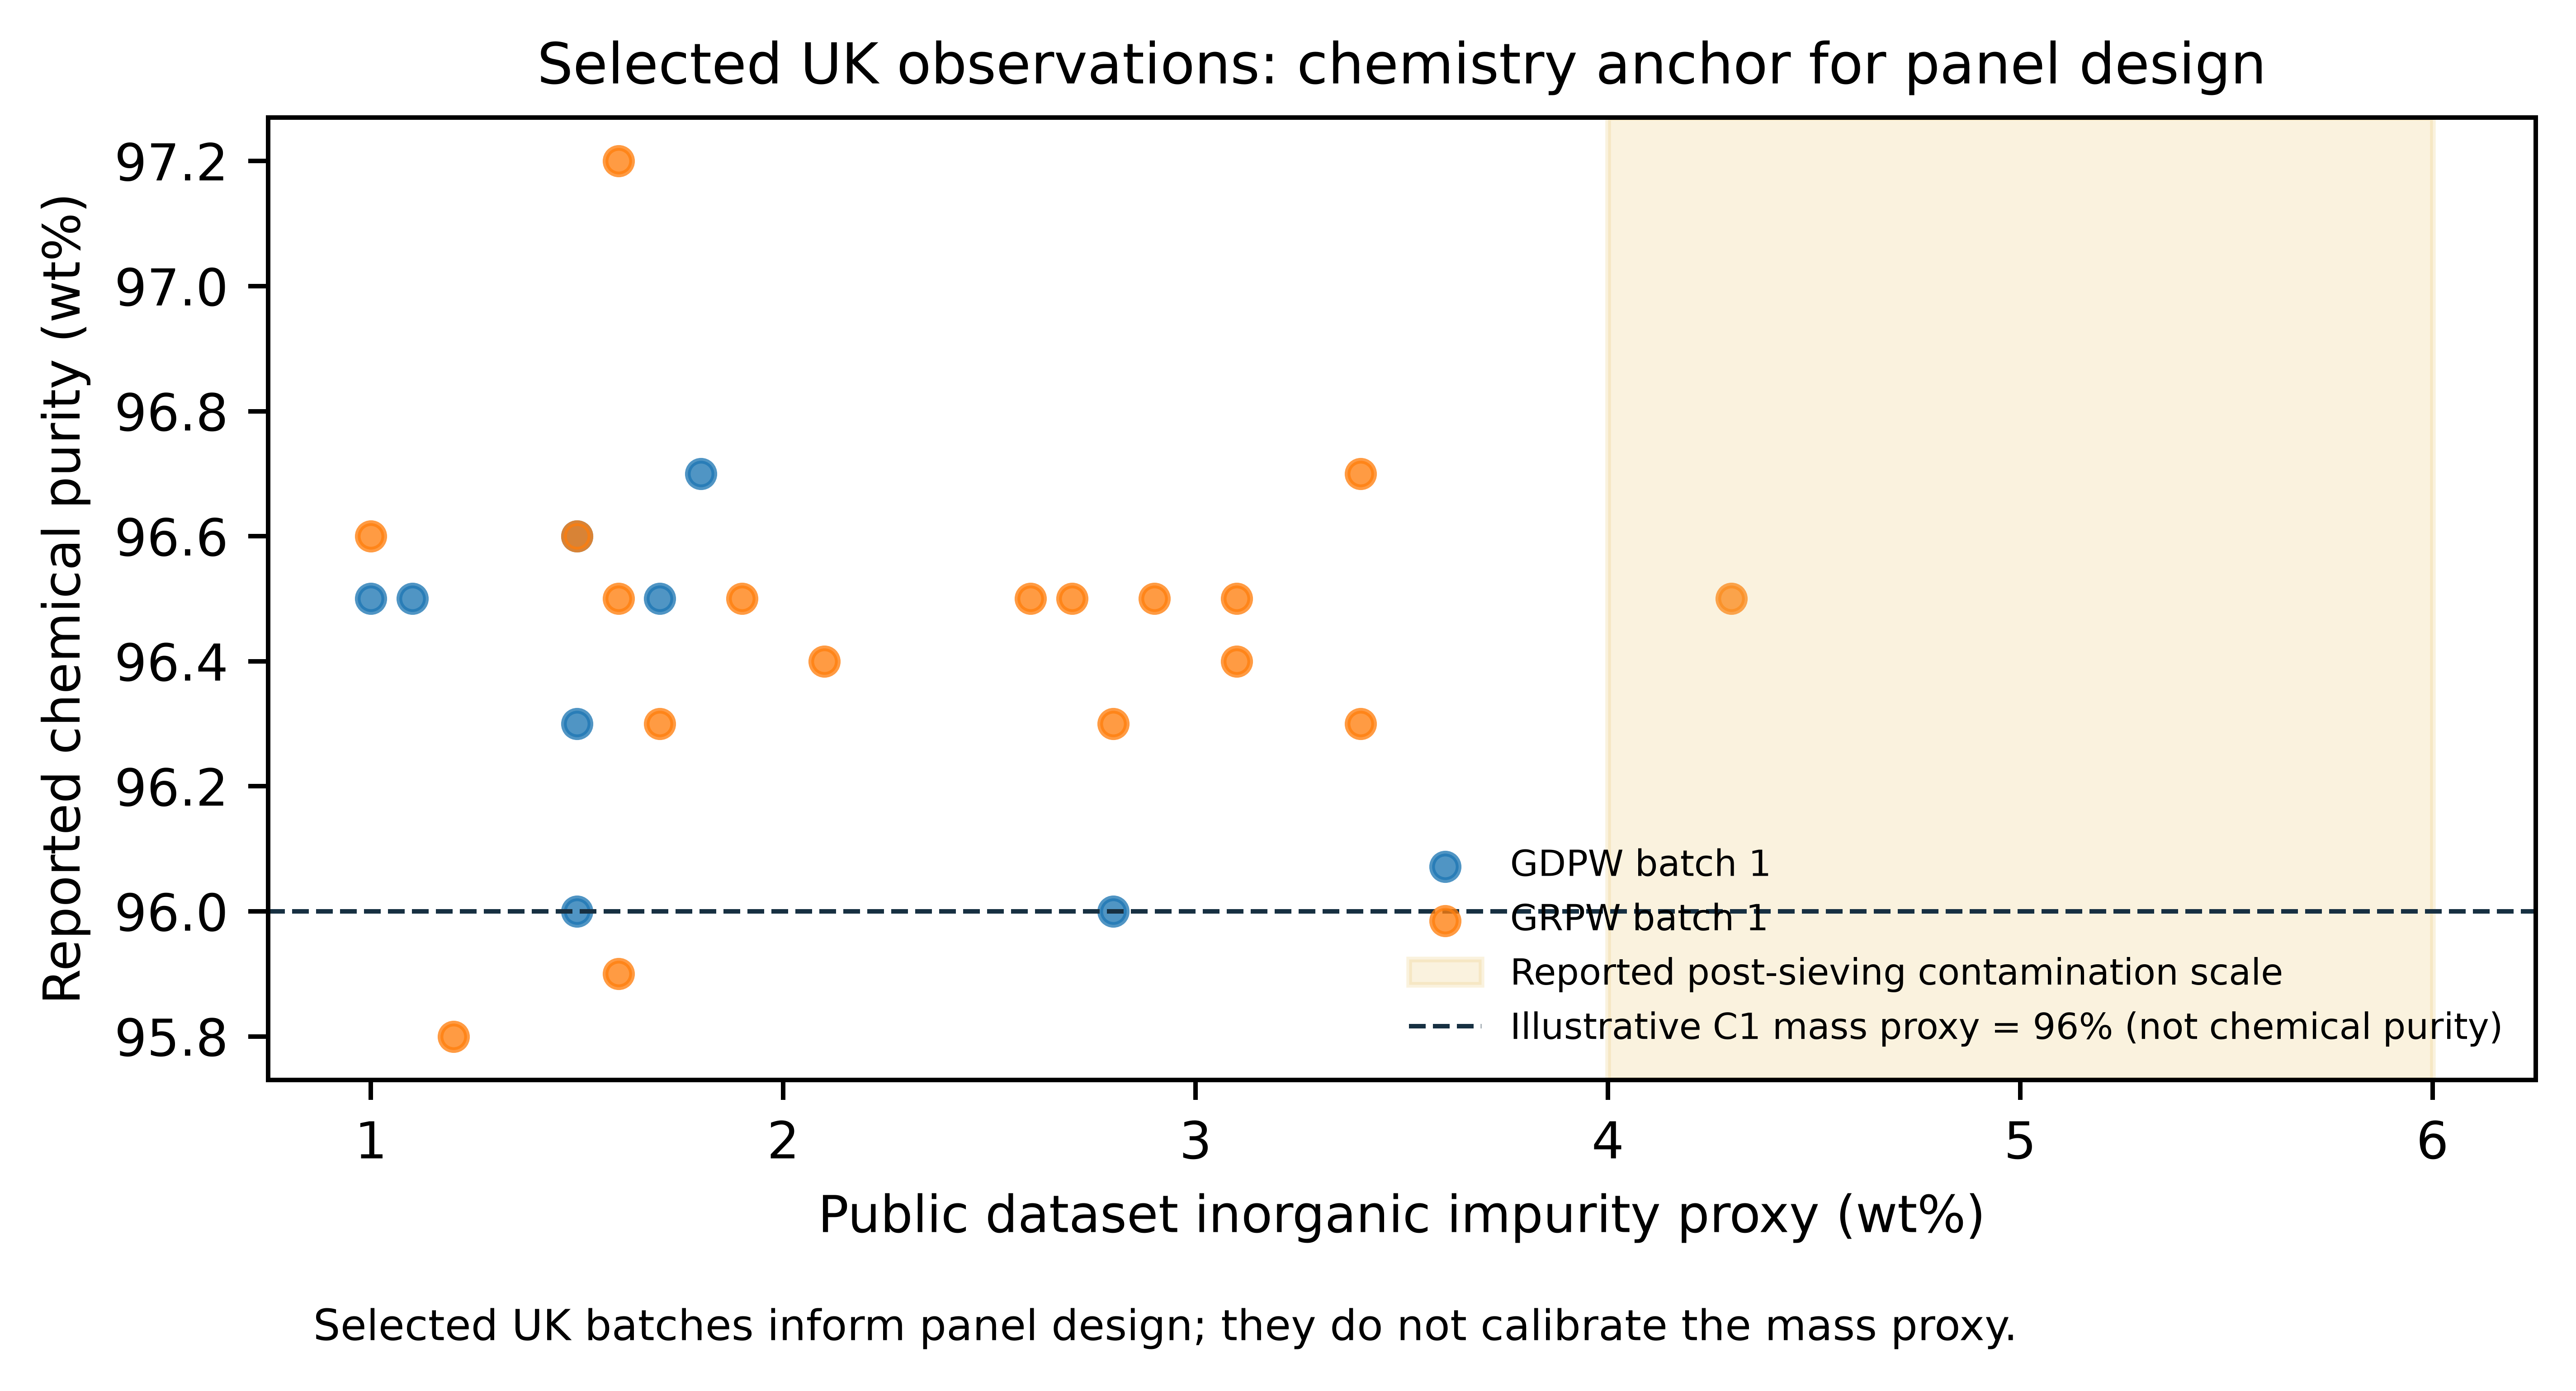
\includegraphics[width=0.96\textwidth]{Fig4_public_anchor_evidence.png}
\caption{Selected UK public observations as a module specific external anchor}\label{fig:public-anchor}
\end{figure}



\subsection{Direct energy components}\label{direct-energy-components}

The open process inventory contains all three reported energy components: 60.35 kWh electricity, 13.59 m3 natural gas and 0.90 L diesel per tonne of process product. The electricity component calculated with the dated JRC factors ranges from approximately 1.62 kg CO2 equivalent per tonne product in Sweden to 52.93 kg in Poland. Figure 5 displays the direct inventory and representative electricity component results. This gives the screening model a traceable process energy layer for later route comparison, but it is an inventory field for an operational record rather than a quantified net climate benefit.

The JRC 85 kg CO2 equivalent per tonne benchmark, with its published variation, remains an external context value and is kept separate from the direct electricity component because the functional unit and substitution boundary differ. The process inventory is selected and Spanish, while the electricity factors are country level and end in 2021. A route comparison that includes transport, water, wastewater, rejects, infrastructure, fuel factors, product substitution and a common functional unit is outside the present inventory.

\begin{figure}[htbp]
\centering
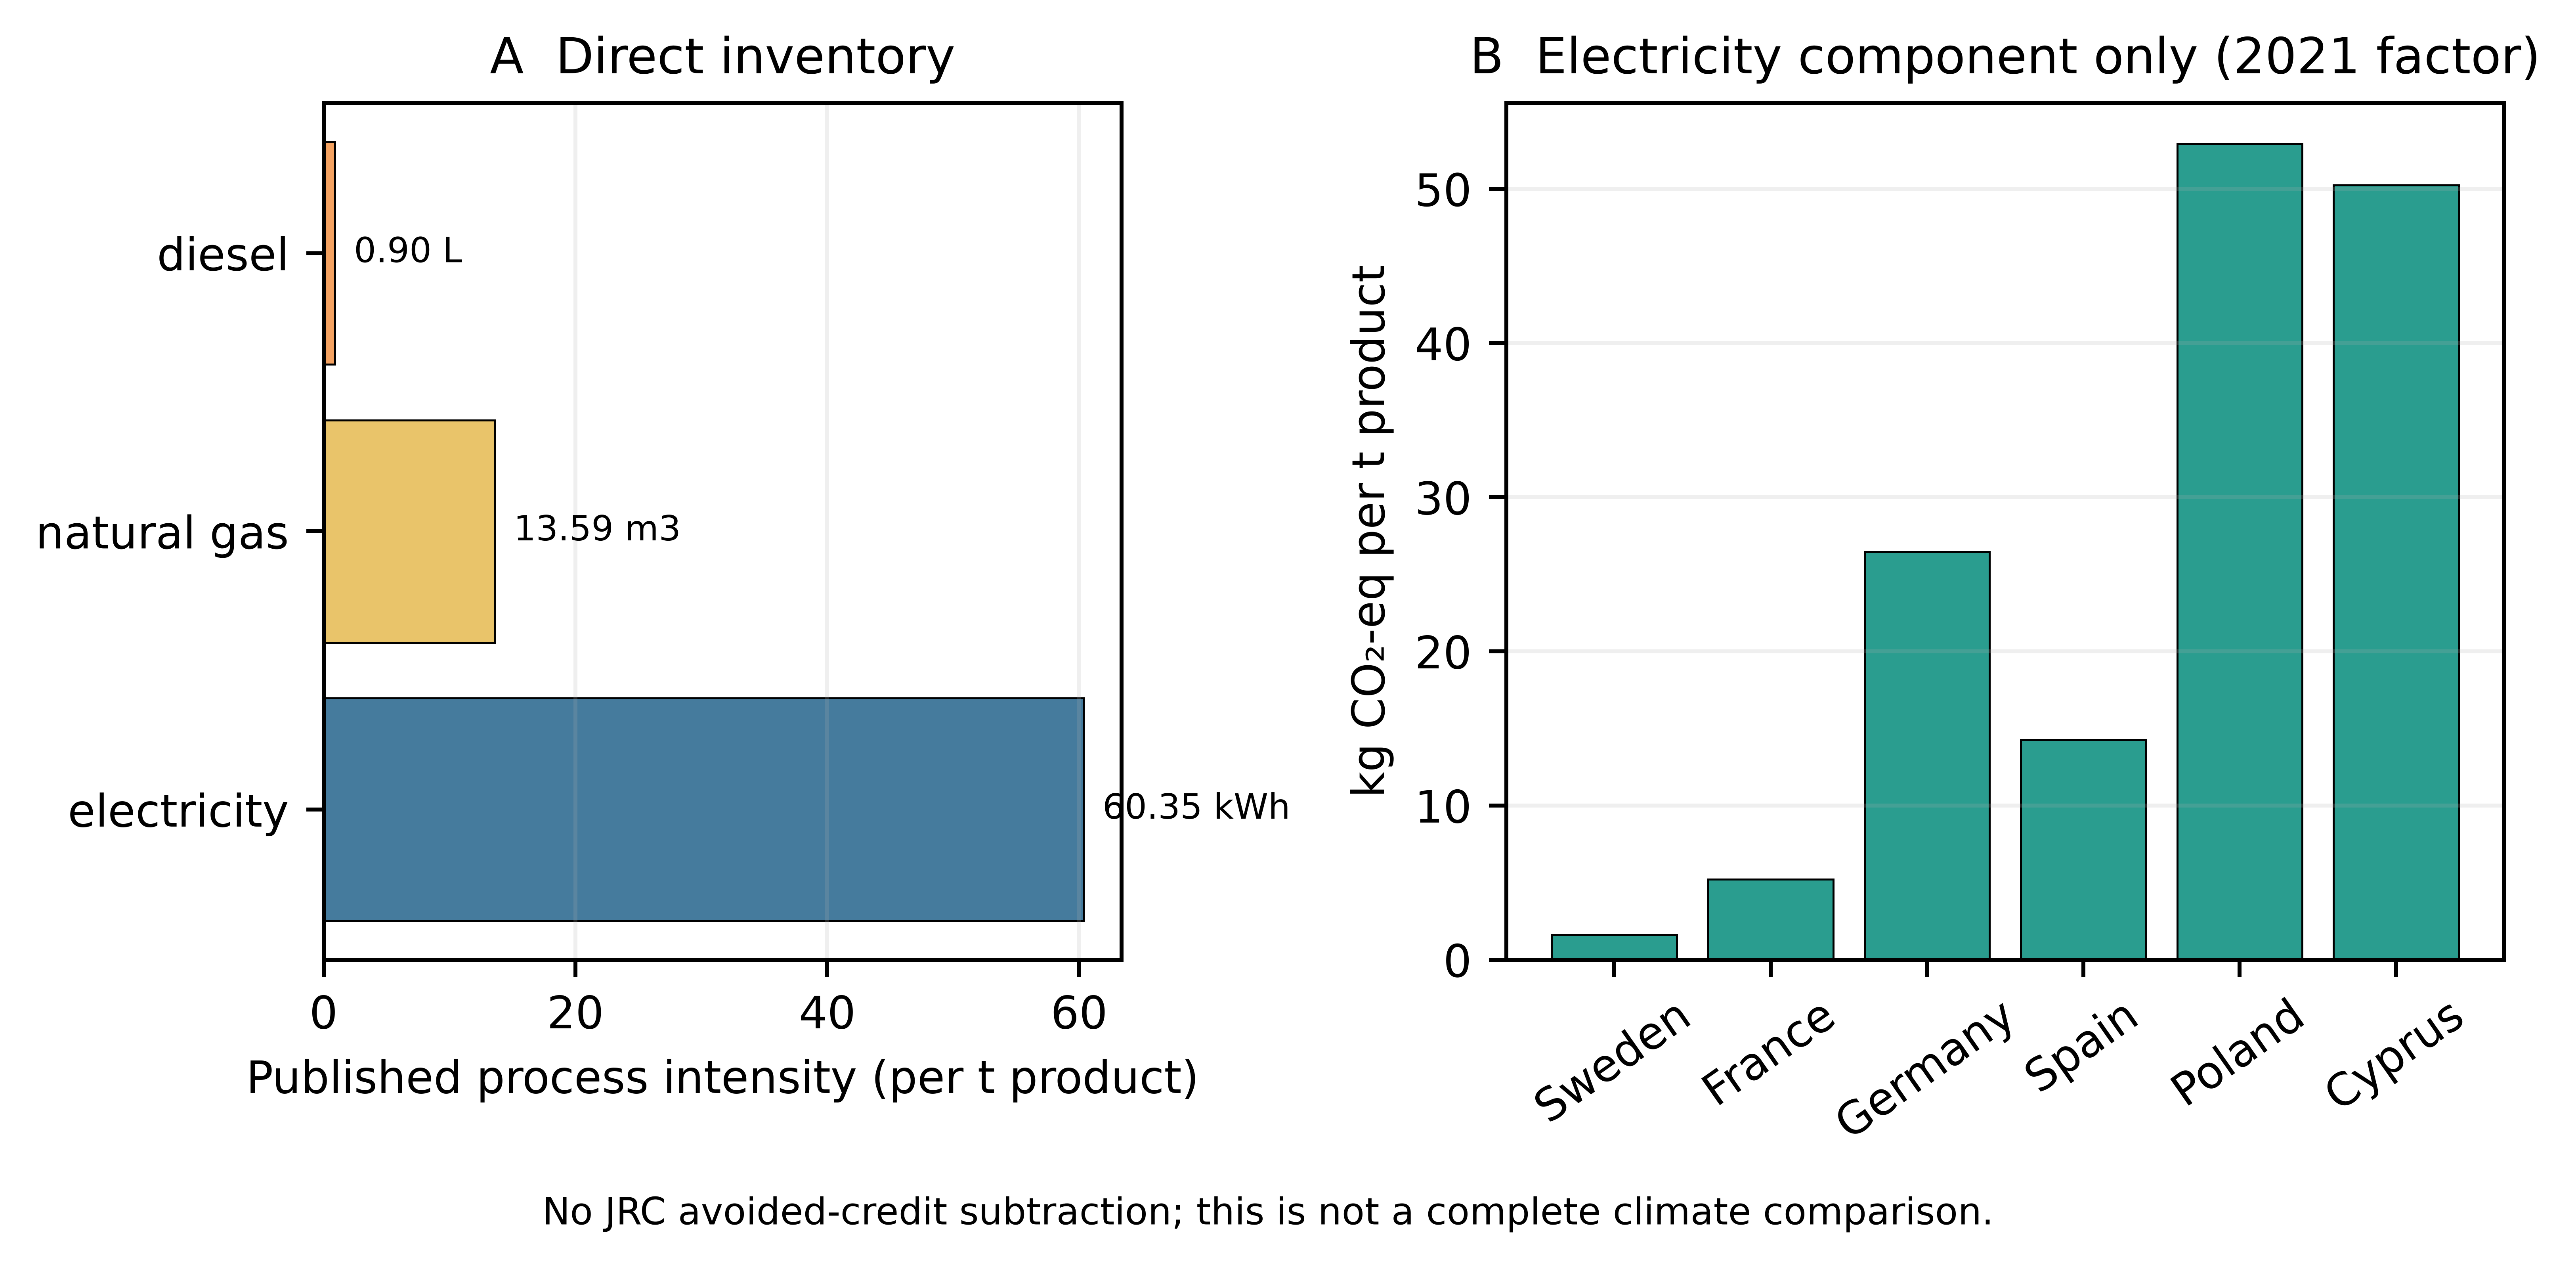
\includegraphics[width=0.96\textwidth]{Fig5_direct_energy_components.png}
\caption{Direct process energy inventory and electricity component sensitivity}\label{fig:energy-components}
\end{figure}



\section{Discussion}\label{discussion}

\subsection{Operational outputs for facility records}\label{operational-outputs-for-facility-records}

The analysis delivers an operational decision structure comprising four linked recordkeeping steps:

\begin{itemize}

\item
  \textbf{Record identity and basis.} Register the source, material stage, input denominator, dry basis, process boundary and hazard information before interpreting a yield or quality value.
\item
  \textbf{Separate safety from visible contamination.} Send a confirmed hazard to an authorized safety route; send visible nonhazardous contamination to a pretreatment and recheck branch rather than treating the flag as automatic final rejection.
\item
  \textbf{Apply the mass triage screen.} Use the registered dry mass balance and component proxies to identify stable, boundary and unresolved cases. C0 passes the primary mass triage in all 32 registered corners, with 662.592 to 739.200 kg dry gypsum equivalent.
\item
  \textbf{Use the product chemistry checklist.} For C0 to C2, record five fields on the product basis required by the receiving route: CaSO4 or chemical purity, TOC, product moisture, chloride or relevant salts, and pH.
\end{itemize}

This makes a label such as clean an auditable registered interval rather than a subjective description. The decision log records the input basis, registered values or ranges, missing fields, routing reason and next action. When a matched product record is available, the same schema provides the fields needed for a qualified recovery calculation or a consistent environmental inventory. The present output is therefore a measurement and routing specification for subsequent product verification.

\subsection{Measurement and treatment are separate pathways}\label{measurement-and-treatment-are-separate-pathways}

The public model addresses the information pathway:

\[
\text{detection}\rightarrow\text{information}\rightarrow\text{routing decision}.
\]

The corresponding physical treatment pathway is:

\[
\text{pretreatment}\rightarrow\text{composition change}\rightarrow\text{qualified product output}.
\]

The distinction matters for C2. A visible nonhazardous contaminant identifies a route hypothesis for stronger paper separation, secondary screening or drying. C2 is consequently reported as a pretreatment candidate whose post treatment outcome must be recorded with the same mass and product fields. The public model supplies the route hypothesis and recheck requirement; a treatment effect would require a separate matched process record.

For operators, this separation prevents two common interpretation errors: treating a measurement as if it were a treatment, and treating a mass proxy as if it were a chemical acceptance result.

\subsection{Interval interpretation and algebraic implications}\label{interval-interpretation-and-algebraic-implications}

The 32 corners define an interval feasibility envelope. The C0 32 of 32 result reflects the registered rectangle and the diagnostic triage limits, while the C1 boundary reflects its registered bounds and the same limits. The envelope is a transparent stress test and provides a reference against which future matched batch records can be compared; measured joint feasible regions can then replace the rectangular bounds.

The algebra also identifies the current model's information structure. Yield multiplies all dry output components and therefore affects quantity, whereas the dry ratios are determined by the retained fractions. In an operating process, yield may be recorded alongside particle size, separation selectivity, reject composition, energy and product specification outcome; those fields define the next data requirements for extending the model. The corner fraction is interpreted as a feasibility fraction within the registered envelope.

The tool is a deterministic pre screening rule system for public records. Its value is traceability: two users applying the same registered basis and the same routing rule should obtain the same next action, while any change in a threshold, denominator or source record remains visible in the decision log.

\subsection{Environmental boundary and scope of country comparison}\label{environmental-boundary-and-scope-of-country-comparison}

The environmental result is a direct inventory sensitivity. The 2021 electricity factor is retained because it is the latest common year in the selected JRC workbook and because the factor type is recorded. A defensible route comparison uses the same input, product function, process stages, fuel and electricity accounting, transport, rejects, water, wastewater and substitution relationship for the baseline and treatment routes.

The EU W121 statistics remain macro construction and demolition waste context rather than batch quality data. Country scenarios sharing C1 parameters are applications of one common model. The national electricity component is therefore retained as an optional sensitivity table rather than a European recycling map.

\subsection{Public record consistency checking for deployment}\label{public-record-consistency-checking-for-deployment}

External public-record consistency checking is the appropriate deployment check for this model. An eligible observation has a traceable source, material stage, denominator and reported quality field in the original paper, data deposit or official record. Study family, preprint, article and data deposit are linked before observations are counted, and interval-defining rows are labelled as calibration evidence rather than a separate check.

Applying the fixed screen without re-estimating its thresholds yields an external consistency check. The check reports eligible records, source families, countries, material stages, matched fields and missing fields, followed by agreement or disagreement between the model route and the reported source category. The selected UK observations used in this paper are a module specific public anchor because they inform the contamination trajectory; the source ledger records this role explicitly.

The accompanying public-data package provides an extraction schema, source-linkage fields, a duplicate-family audit and an analysis script. The deployment contribution is a reproducible public-record protocol for extending the screen when matched facility or public observations become available. Its current evidence basis is computational and public-record based.

\subsection{Limitations}\label{limitations}

Scope Box 1 defines the boundary of the present public-data outputs. The tool supports record standardization, triage and measurement planning within the declared proxy screen. The registered scenarios are not linked to a harmonized independent public batch panel, C2 has no observed post treatment outcome in the public record, the direct energy inventory is incomplete for a route LCA, and the public record contains no harmonized price, capital, labor or acceptance contract data for LCC.

\section{Conclusions}\label{conclusions}

This study delivers a public data decision support tool for batch level triage and pretreatment routing of post consumer gypsum plasterboard. It converts incomplete source records into a dry basis mass balance, an explicit safety first route and a five field chemistry checklist. The registered parameter set produces 662.592 to 739.200 kg dry gypsum equivalent across the 32 registered C0 corners, and all corners pass the primary mass triage screen. The 0.84 composition share and the 0.80 to 0.88 German process range use different denominators and are retained as separate, traceable variants.

The operational outputs are explicit: C0 can be routed consistently to chemistry confirmation, C1 remains a boundary case, C2 is sent to pretreatment and recheck, and C3 exits at the hazard gate. Product acceptance is represented by the five product basis fields specified for the receiving route, while direct electricity, gas and diesel components are reported with their source denominators. The published net climate benchmark remains an external context value.

The practical value is a common decision log for facility records, supplier communication and public data harmonization. It makes the denominator, missing fields and next action explicit, and places macro flows, mass proxies and climate context in their appropriate roles alongside product basis evidence. Qualified recovery can be estimated when a public, traceable batch record contains matched input and product chemistry fields together with the route outcome.

\section*{Acknowledgements}

The authors acknowledge the public data producers, open research repositories, European institutions and technical organizations cited in the reference list. No unpublished facility data, field samples, laboratory campaign or human-subject data were used.

\bibliography{references}

\section*{Declarations}

\subsection*{Funding}

No funding was obtained specifically for this computational study.

\subsection*{Competing interests}

The authors declare no competing interests. Source-level interests disclosed in cited studies are retained in the source audit record and are not treated as independent validation.

\subsection*{Ethics approval}

Not applicable. This computational study used public records and public datasets only and involved no human participants, animals, personal data or biological material.

\subsection*{Consent to participate}

Not applicable.

\subsection*{Consent to publish}

Not applicable.

\subsection*{Data availability}

The reproducibility package contains the public parameter registers, data dictionary, derived CSV tables, analysis scripts, figure scripts and publication figures. Publisher hosted PDFs and other third party files are not redistributed; source URLs and source locators are supplied for reacquisition, and source data remain subject to their respective reuse terms. The package is openly available at https://doi.org/10.5281/zenodo.22648030, with the versioned source repository at https://github.com/williamjay1/gypsum-plasterboard-public-data-screening.

\subsection*{Code availability}

The analysis and figure scripts are included in the accompanying reproducibility package at https://doi.org/10.5281/zenodo.22648030 and https://github.com/williamjay1/gypsum-plasterboard-public-data-screening, and are released under the MIT License. The package includes the code, public data working tables and derived results needed to reproduce the reported tables and figures.

\subsection*{Authors' contributions}

Junjie Zhang led public data curation, computational implementation, validation and initial drafting. Yujue Cao contributed to study supervision, methodological interpretation and critical revision. Both authors contributed to the study conception, approved the final manuscript and accept responsibility for its content.

\subsection*{Generative AI use}

OpenAI Codex (GPT-5) was used for Python code drafting and English language editing during manuscript preparation. The authors reviewed and verified all analytical decisions, numerical results, interpretations and substantive claims against the cited public sources, equations and reproducibility files, and take full responsibility for the final manuscript.

\begin{appendices}

\section{Public batch observation extraction schema}\label{appendix-a.-public-batch-observation-extraction-schema}

For every public batch-level observation, record a unique observation identifier, the source publication or data-deposit identifier, source family, country or region, material stage, feed description, reported denominator, collection or experiment description as reported by the source, and the exact table, figure or page locator. The source record must distinguish reported fact, author interpretation and missing field. Do not reconstruct a missing dry mass, product yield or chemical result from a proxy unless the reconstruction rule is explicitly registered.

Where reported, extract input and output mass basis, moisture, board-bearing fraction, paper, coating, wood, mineral and metal fractions, hazard flag, CaSO4 or chemical purity, TOC, soluble salts, pH, visible contamination, energy, water, process condition, reject destination and reported acceptance outcome. These fields form an evidence schema; they are not a request for new sampling or laboratory work.

Link preprints, journal articles, supplementary files and data deposits that describe the same study family. The same observation must receive one canonical identifier. Observations without a traceable denominator or stage remain partial records and cannot be used to calibrate the mass balance.

\section{Public-data external consistency protocol}\label{appendix-b.-public-data-external-consistency-protocol}

The external check uses only records that were publicly available and traceable in the source ledger. First, freeze the model registry, routing order and threshold definitions. Second, search for public records from source families not used to set the specific parameter interval being checked. Third, de-duplicate study families and retain the source locator for every value. Fourth, apply the frozen screen without refitting thresholds to the extracted record. Fifth, compare the predicted route with the reported source category only where the denominators, stage and quality definition are comparable.

Report the number of eligible observations, independent source families, countries, material stages, matched fields, missing fields and excluded duplicate or non-comparable records. Report agreement and disagreement as descriptive external consistency results with source-level provenance. Do not call the result a treatment effect, a product certification, an EU prevalence estimate or a human-subject result. The UK observations used in this manuscript are a module-specific public anchor and are not counted as independent validation of the full screening rule because they informed the contamination trajectory. No field sampling, laboratory campaign, randomisation or participant data are used.

\end{appendices}

\end{document}
